\documentclass[12pt, a4paper]{article}

\title{\textsc{Linear Algebra} Assignment 2 Report}
\author{110062219 翁君牧}
\date{\today}

\usepackage{xeCJK}
\usepackage{amsmath}
\usepackage{amssymb}
\usepackage{caption}
\usepackage{subcaption}
\usepackage{tikz}
\usepackage{pgfplots}
\usepackage{listings}
\usepackage{hyperref}
\usepackage{booktabs}
\usepackage{biblatex}
\usepackage{longtable}

\lstset{
	breaklines=true,
	basicstyle=\ttfamily,
}

\definecolor{nthu}{HTML}{7F1084}

\addbibresource{A2_110062219.bib}

\begin{document}

\maketitle

\tableofcontents
\listoffigures

\section{Different Selections of Equations}

It's obvious that there are \(\binom{14}{11}=364\) combinations. As a consequence, it's not hard to enumerate all selections and measure, compare their performances. I allocated a full single node on \textbf{Taiwania 3} to run the \textsf{Jupyter} server.

Each one was iterated \(10000\) times in loop and repeat \(5\) times. We should be cautious that some combinations are \emph{singular} which means that it couldn't lead to a solution.

The \(\min\)imum was \(9.08\mu s\) whereas the \(\max\)imum being \(9.84\mu s\). Note that even though the amount of iterations had been increased again and again, the result still varied and diverged. That is to say, we failed to obtain an optimal combination that is ensured to yield the best result all times. Still, we could see that it seems that if we select rows \(8\), \(13\) then the result have a tendency to be a bit better.

\section{Using \itshape Linear Least Square}

We're asked to try to call \texttt{numpy.linalg.lstsq()} to solve the overdetermined system. I also iterated it for \(10000\) times in loop and repeat \(5\) times so as to do comparison.

We could find that the CPU time consumed by \emph{linear least square}, \(38.9\mu s\), was about \(4\) times the slowest one in different selections of equations. So why's the reason? I sought the \href{https://numpy.org/doc/stable/reference/generated/numpy.linalg.lstsq.html}{documentation}\footfullcite{lstsq} of \texttt{numpy.linalg.lstsq()} and found that first the function returns more additional informations, such as \emph{residual sum of squares (or \emph{the difference between the measured and projected point})}, \emph{rank} and \emph{singular value}s of $A$. Moreover, it also said that: \begin{quote} If there are multiple minimizing solutions, the one with the smallest \(2\)-norm \(||x||\) is returned. \end{quote}

For the purpose of doing so, the matrix needs be examined and sometimes solved by means of \textbf{Pseudo Inverse}, while there are faster approach such as \textbf{QR decomposition}.

Nevertheless, the returned matrix of \texttt{numpy.linalg.lstsq()} tended to be more stable.

\section{Take a Photo of a Rectangular Object}

Figure \ref{fig:box_org} is a shoe box I chose of size \(33\) by \(18.5\) by \(12\) cm. that is suitable for this task. The 2D coordinates of its vertices is labeled on Figure \ref{fig:box_marked} by hands.

\begin{figure}[htbp]
\centering
\begin{subfigure}{.45\linewidth}
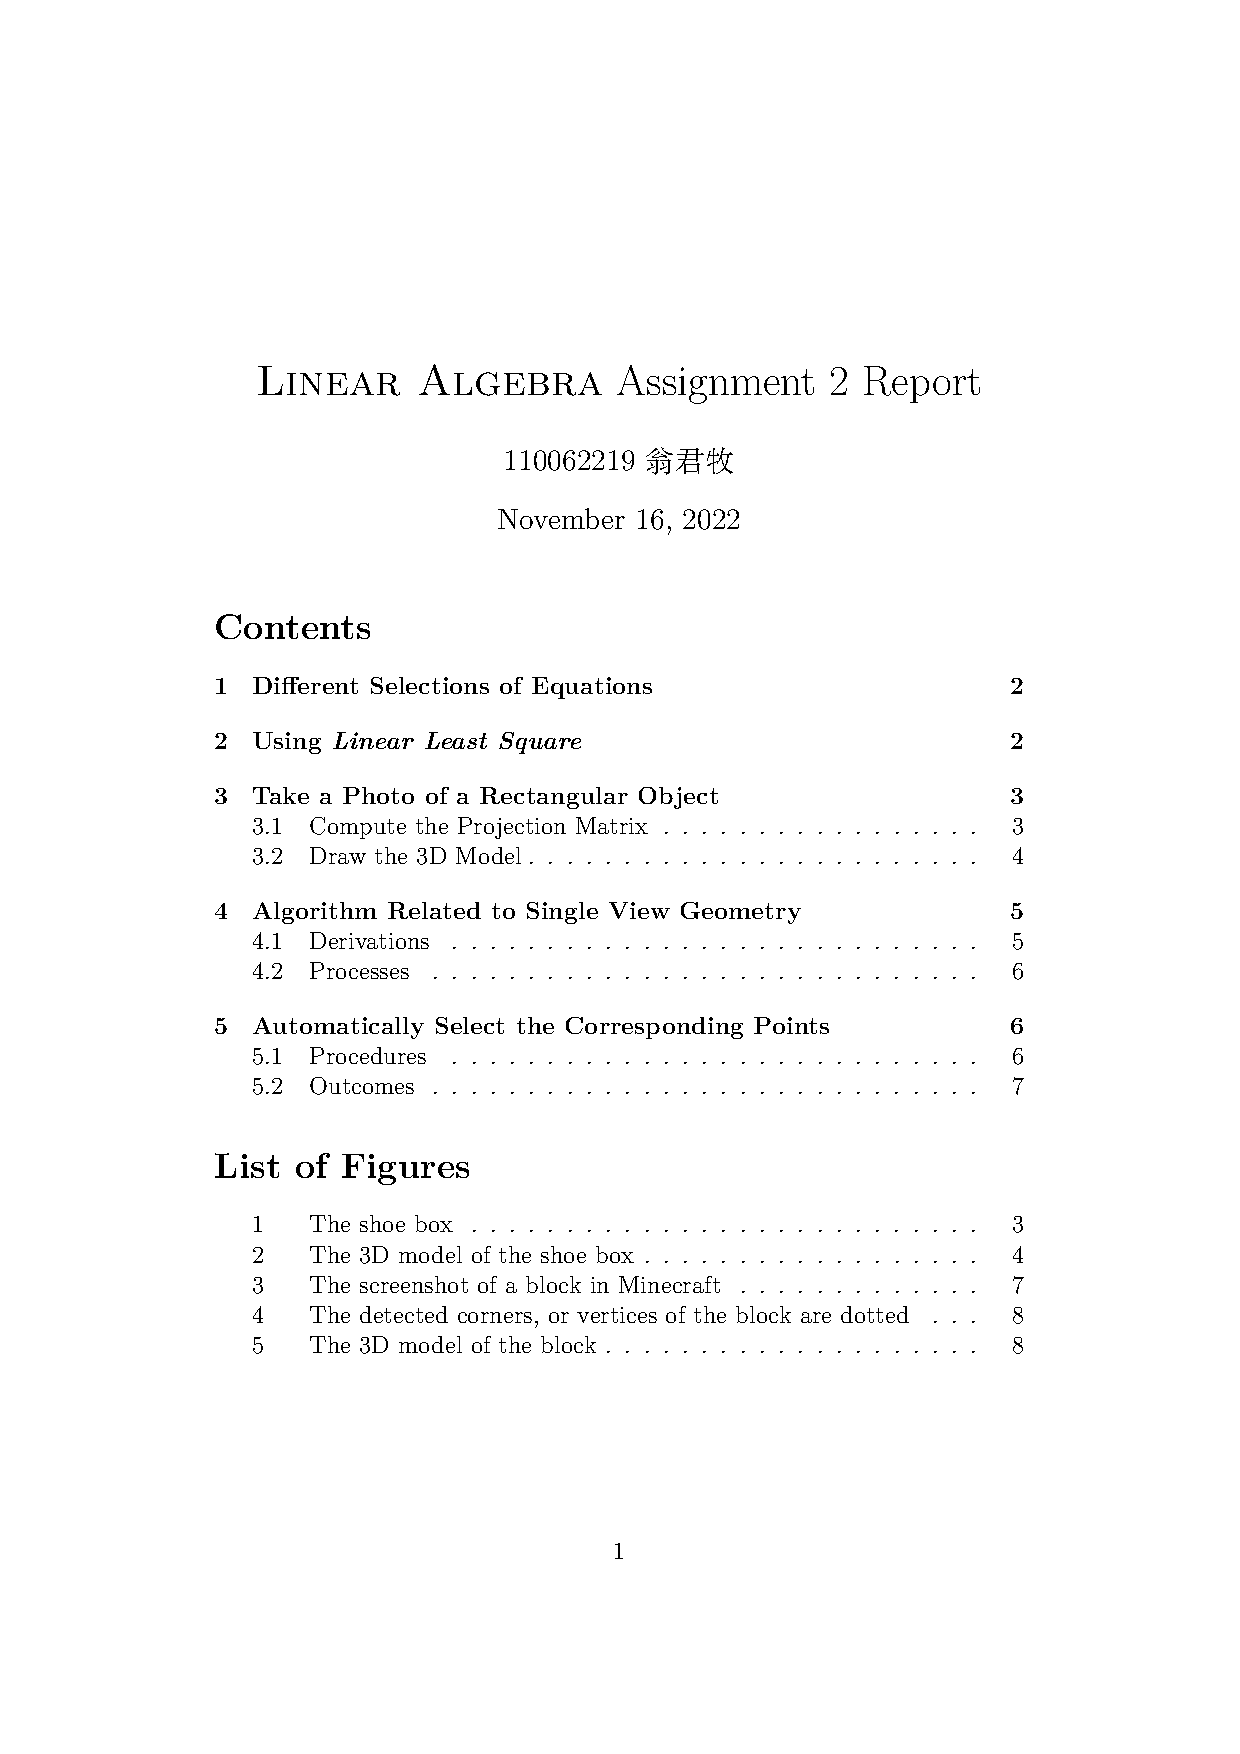
\includegraphics[width=\linewidth]{A2_110062219.JPG}
\caption{Original photo}
\label{fig:box_org}
\end{subfigure}
\begin{subfigure}{.45\linewidth}
\includegraphics[width=\linewidth]{A2_110062219_marked.JPG}
\caption{Marked by hands}
\label{fig:box_marked}
\end{subfigure}
\caption{The shoe box}
\label{fig:box}
\end{figure}

Despite the fact that the box isn't cubic, we could still project the box to the unit cube in the first octant since we could consider the project matrix also performs the \emph{scaling} linear transformation. I constructed Table \ref{tab:box} of the corresponding of 3D points between 2D also by hands.

\begin{table}[htp]
\centering
\caption{Corresponding of 3D Points Between 2D}
\begin{longtable}[]{@{}cc@{}}
\toprule()
3D & 2D \\
\midrule()
\endhead
(0, 0, 1) & (32.5, 66.5) \\
(0, 1, 0) & (55, 30.5) \\
(0, 1, 1) & (27, 47.5) \\
(1, 0, 0) & (109.5, 72) \\
(1, 0, 1) & (92, 102.5) \\
(1, 1, 0) & (115.5, 52) \\
(1, 1, 1) & (94.5, 83) \\
\bottomrule()
\end{longtable}
\label{tab:box}
\end{table}%

\subsection{Compute the Projection Matrix}

By referring the template codes providing, we have the projection matrix computed:

\[
P=\begin{pmatrix}
 27.32705956 & -12.59046806 & -27.92830833 & 59.3337975 \\
  7.42640673 & -24.90881322 &   7.17919923 & 50.8301141 \\
 -0.20857665 &  -0.15012128 &  -0.15302608 &  1.
 \end{pmatrix}
 \]

\subsection{Draw the 3D Model}

Calling the function provided in template codes, we could obtain the 3D model of the shoe box shown in Figure \ref{fig:box_model}.

\begin{figure}[htbp]
\centering
\includegraphics[width=\linewidth]{shoe_box_model}
\caption{The 3D model of the shoe box}
\label{fig:box_model}
\end{figure}

\section{Algorithm Related to Single View Geometry}

\subsection{Derivations}

When it comes to camera calibration of an image, there are 3 coordinate systems involved --- camera (2D or 3D), image and world.

On the image plane, the points are mapped to 2D camera coordinates by the \textbf{camera calibration matrix} $C$, which is upper-triangular and determined by the scaling $\alpha$ in the image in the two directions and the principal point $(u_0,v_0)$, $$\begin{pmatrix}u\\v\\1\end{pmatrix}=\begin{pmatrix}\alpha_u&0&u_0\\0&\alpha_v&v_0\\0&0&1\end{pmatrix}\begin{pmatrix}x_c\\y_c\\f\end{pmatrix}$$.

By \emph{pinhole imaging \emph{and} similar triangles}, we could found the perspective projection from 2D camera to 3D $\begin{pmatrix}x_c\\y_c\\f\end{pmatrix}=\lambda\begin{pmatrix}X_c\\Y_c\\Z_c\end{pmatrix}$, where $\lambda=\frac{f}{Z_c}$, or $$\begin{pmatrix}x_c\\y_c\\f\end{pmatrix}=\begin{pmatrix}I&\mathbf{0}\end{pmatrix}\begin{pmatrix}X_c\\Y_c\\Z_c\\1\end{pmatrix}$$ in \emph{homogeneous system}.

The relation between the camera and world 3D coordinates could be expressed as $\mathbf{X_c}=R\mathbf{X_w}+T$, i.e., $$\begin{pmatrix}X_c\\Y_c\\Z_c\\1\end{pmatrix}=\begin{pmatrix}R&T\\0^T&1\end{pmatrix}\begin{pmatrix}X_w\\Y_w\\Z_w\\1\end{pmatrix}$$, where $R$ is a $3\times3$ rotation matrix.

As a consequence, we have the transformation between the image and the world coordinate: $$\begin{pmatrix}u\\v\\1\end{pmatrix}=C\begin{pmatrix}I&\mathbf{0}\end{pmatrix}\begin{pmatrix}R&T\\0^T&1\end{pmatrix}\begin{pmatrix}X_w\\Y_w\\Z_w\\1\end{pmatrix}=C(R|T)\begin{pmatrix}X_w\\Y_w\\Z_w\\1\end{pmatrix}$$. Thereby we define the $3\times4$ \textbf{projection matrix} $P=C(R|T)$, where $\mathbf{x}=P\begin{pmatrix}\mathbf{X}\\1\end{pmatrix}$. The null-space of $P$ is the optical centre of the camera.

\subsection{Processes}

By enough correspondences, i.e., at least 6 points, \textbf{projection matrix} $P$ could be resolved. Subsequently, we should factorize $P$ back to \textbf{camera calibration matrix} $C$, $R$ and $T$.

The first $3\times3$ submatrix of $P$ is the product of an upper triangular matrix $C$ and rotation matrix $R$. Thus by \textbf{QR decomposition}, $C$ and $R$ could be solved. Then for the remaining part, we could find that $T=C^{-1}\begin{pmatrix}p_{14}\\p_{24}\\p_{34}\end{pmatrix}$.

Note that $C$ solved by this manner, we would have an additional entry $k$ at $(1,2)$, indicating the \emph{skew coefficient}.

\section{Automatically Select the Corresponding Points}

\subsection{Procedures}

I found this
\href{https://docs.opencv.org/3.4/d4/d8c/tutorial_py_shi_tomasi.html}{document}\footfullcite{opencv} being of help toward this task online, looked into the computer vision library \textbf{OpenCV} and made use of the function \texttt{cv2.goodFeaturesToTrack()} to apply \emph{Shi-Tomasi} algorithm\footfullcite{st} to find desired corners in the image.

First I preset the threshold and minimum distance, transformed the image into gray scale and find the 7 most-likely corners, or vertices. Then, I assume that the rightmost point on 2D must be \((0,0,1)\) in 3D, says \(pa\) , the topmost one must be \((0,1,0)\), says \(pb\) and the bottommost and the right most must be \((1,0,0)\) and \((1,0,1)\), says \(pc\) and \(pd\) respectively. For the remaining 3 points, if its x-distance to \(pa\) is less than the one o the minimum of \(pa\), \(pc\), then I assume it must be \((0,0,0)\)
in 3D. Else if its x-distance to \(pd\) is less than the one to the maximum of \(pa\), \(pc\), then I assume it must be \((0,0,0)\) in 3D. Else if its x-distance to \(pa\) is less than the one to the minimum of \(pa\), \(pc\), then I assume it must be \((0,1,1)\) in 3D. Otherwise, I assume the point to be \((1,1,1)\) in 3D.

\subsection{Outcomes}

Nevertheless, I tried several photos in real-life including the one for the third question yet their results were all quite awful. As a consequence, I turned to some simple 3D model images generated by some tools and found that my codes worked indeed. Furthermore, I tested a screenshot, shown in Figure \ref{fig:block}, taken in the game Minecraft.

\begin{figure}[htbp]
\centering
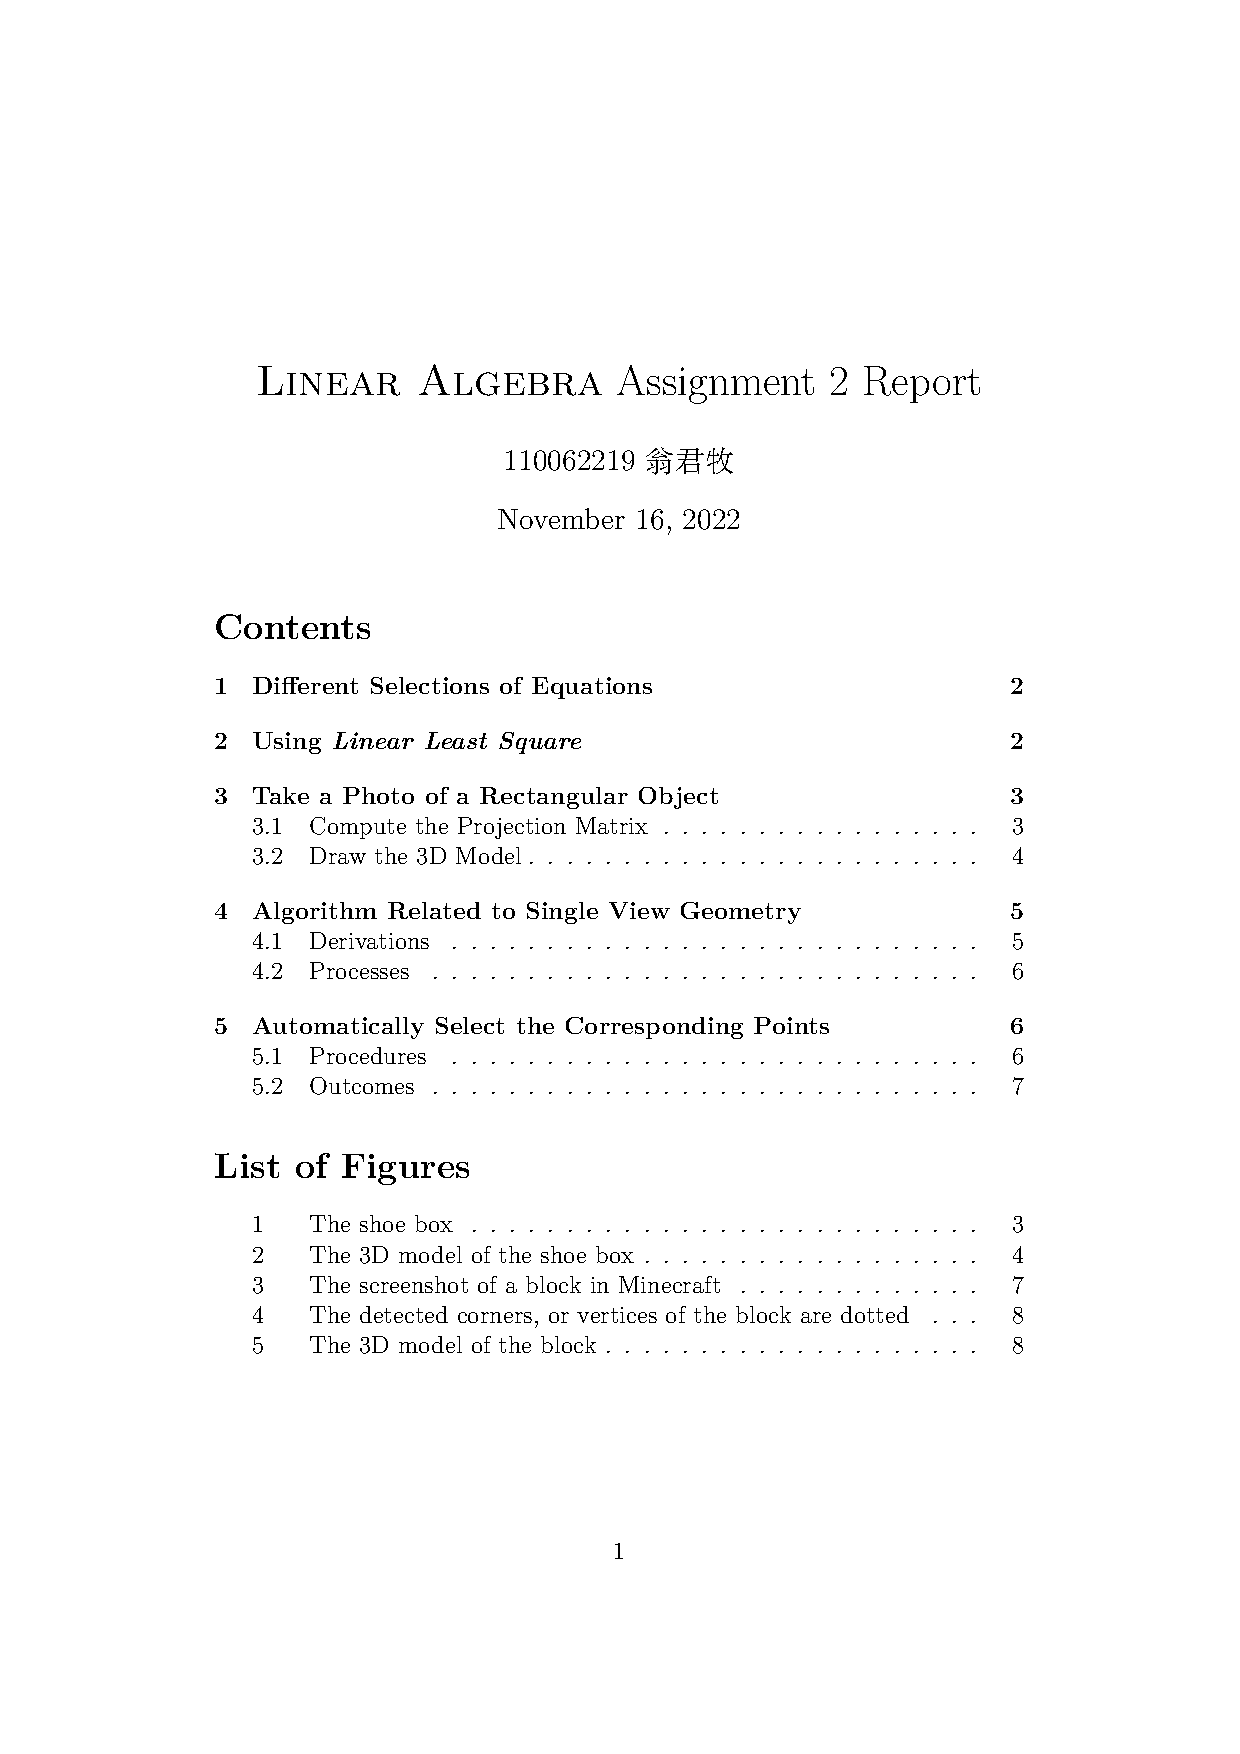
\includegraphics[width=\linewidth]{A2_110062219.png}
\caption{The screenshot of a block in Minecraft}
\label{fig:block}
\end{figure}

I believe that it may be the inevitable vast amount of noises plus the complex inhered informations for the real-life photos such that my codes couldn't give ideal outcome. It might require some additional effort such as proper preprocessing, Gaussian blurring, but it's supposed to be beyond this course, \textsc{Linear Algebra}.

\begin{figure}[htbp]
\centering
\includegraphics[width=\linewidth]{block_corners}
\caption{The detected corners, or vertices of the block are dotted}
\label{fig:block_corners}
\end{figure}

\begin{figure}[htbp]
\centering
\includegraphics[width=\linewidth]{block_model}
\caption{The 3D model of the block}
\label{fig:block_model}
\end{figure}

Although we could see that in Figure \ref{fig:block_corners} the 3D point $(1,1,1)$ wasn't marked precisely, yet in my opinion, the model in Figure \ref{fig:block_model} looked fine enough. And I found that the results might differ, despite the fact that I also tried to fix the selection slice of equations (rows of $A$, $b$). Sometimes the result went quite weird. In these cases, we might need rerun cell 28, 29 again.

\pagebreak

\section*{Acknowledgements}

I thank to \textsf{National Center for High-performance Computing} \textit{(NCHC)} for providing computational and storage resources.

\nocite{*}
\printbibliography

\end{document}
